\documentclass[tikz,border=4pt]{standalone}
\begin{document}
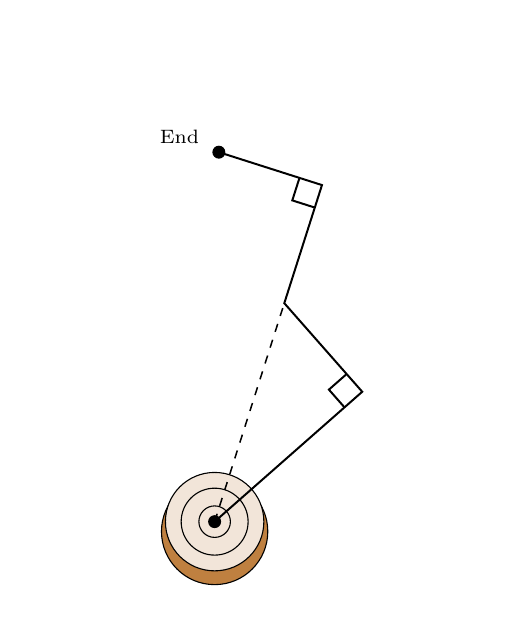
\begin{tikzpicture}[x=.025cm,y=-.025cm]
\path[use as bounding box] (0,0) rectangle (230,290);
\path[draw=black,fill=brown] (95,256) circle[radius=0.675cm];
\path[draw=black,fill=brown!20] (95,251) circle[radius=0.625cm];
\path[draw=black,fill=brown!20] (95,251) circle[radius=0.425cm];
\path[draw=black,fill=brown!20] (95,251) circle[radius=0.2cm];
\path[draw=black,fill=black] (95,251) circle[radius=0.075cm];
\path[draw=black,fill=none,line width=0.55pt,dashed] (95,251) -- (130.4,140);
\path[draw=black,fill=none,line width=0.7150000000000001pt] (95,251) -- (170,185) -- (130.4,140) -- (149.542,79.9785) -- (97.1423,63.2672);
\path[draw=black,fill=none,line width=0.7150000000000001pt] (160.9914,192.9275) -- (153.0639,183.919) -- (162.0725,175.9914);
\path[draw=black,fill=none,line width=0.7150000000000001pt] (145.8959,91.4111) -- (134.4632,87.765) -- (138.1093,76.3324);
\path[draw=black,fill=black] (97.1423,63.2672) circle[radius=0.075cm];
\node[inner sep=0pt,font=\scriptsize] at (77.1423,55.2672) {End};
\end{tikzpicture}
\end{document}
